\documentclass{article}
\usepackage{charter}
\usepackage{graphicx}
\graphicspath{ {./images/} }
\usepackage[landscape]{geometry}
\usepackage{float}
\usepackage{tabularx}
\newcolumntype{Y}{>{\centering\arraybackslash}X}
\geometry{left=0mm, top=5mm, right=0mm, bottom=0mm}

% Create new array 
\ExplSyntaxOn
  \NewDocumentCommand{\setarray}{mm}
  {% #1 = name, #2 = items
    \clist_clear_new:c { array_#1_clist }
    \clist_set:cn { array_#1_clist } { #2 }
  }
  
  \NewExpandableDocumentCommand{\getIndex}{mmm}
  {% #1 = name, #2 = row index, #3 = column index
    \clist_item:en
    {
      \clist_item:cn { array_#1_clist } { #2 }
    }
    { #3 }
  }
  \cs_generate_variant:Nn \clist_item:nn { e }
\ExplSyntaxOff

% Import numbers for bingo table
\setarray{arr}{
{1,22,36,50,69},
{2,21,33,54,73},
{3,16,39,48,70},
{15,24,41,55,61},
{12,19,38,60,72},
{9,23,40,59,70},
{14,21,39,55,61},
{2,29,36,46,72},
{15,16,37,49,65},
{8,28,38,54,68},
}


\begin{document}
\thispagestyle{empty}
% Create table using new array
% Set the divider line width to 0.4pt
\setlength{\arrayrulewidth}{0.3pt}
\def\arraystretch{2.5}%
\begin{tabularx}{\textwidth}{c@{\hskip 30px}c}
    \raisebox{-30px}{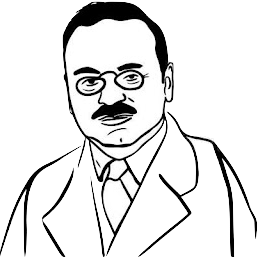
\includegraphics[width=50mm,height=!]{adler2.png}} & \raisebox{-30px}{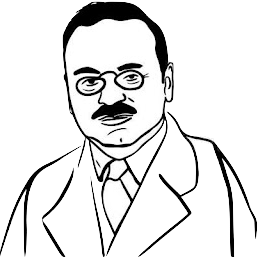
\includegraphics[width=50mm,height=!]{adler2.png}} \\
    \textbf
    \centering
    \resizebox{0.45\textwidth}{!}{%
      \begin{tabularx}{150px}{ |Y|Y|Y|Y|Y| }
        \multicolumn{1}{c}{A} & \multicolumn{1}{c}{D} & \multicolumn{1}{c}{L} & \multicolumn{1}{c}{E} & \multicolumn{1}{c}{R} \vspace*{-0.3em} \\
        \hline
        \getIndex{arr}{1}{1} & \getIndex{arr}{1}{2} & \getIndex{arr}{1}{3}                         & \getIndex{arr}{1}{4} & \getIndex{arr}{1}{5} \\ \hline
        \getIndex{arr}{2}{1} & \getIndex{arr}{2}{2} & \getIndex{arr}{2}{3}                         & \getIndex{arr}{2}{4} & \getIndex{arr}{2}{5} \\ \hline
        \getIndex{arr}{3}{1} & \getIndex{arr}{3}{2} & \hspace*{-1.5mm}\raisebox{-.25\height}{ 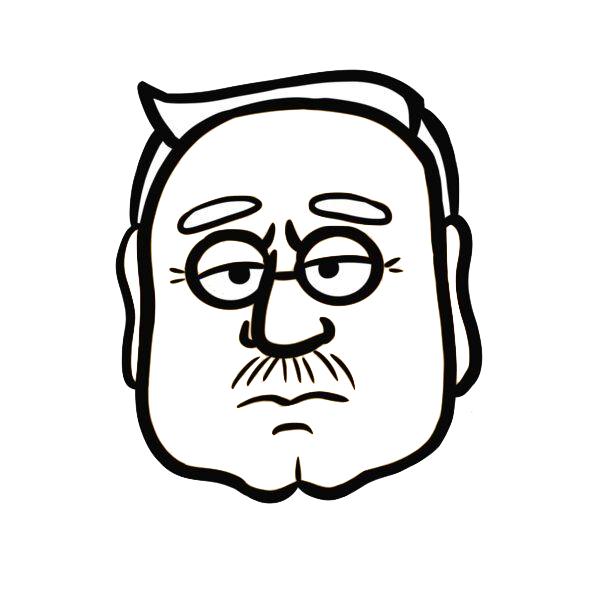
\includegraphics[width=7.5mm,height=7.5mm]{adler1.png} } & \getIndex{arr}{3}{4} & \getIndex{arr}{3}{5} \\ \hline
        \getIndex{arr}{4}{1} & \getIndex{arr}{4}{2} & \getIndex{arr}{4}{3}                         & \getIndex{arr}{4}{4} & \getIndex{arr}{4}{5} \\ \hline
        \getIndex{arr}{5}{1} & \getIndex{arr}{5}{2} & \getIndex{arr}{5}{3}                         & \getIndex{arr}{5}{4} & \getIndex{arr}{5}{5} \\ \hline
      \end{tabularx}%
    } \
&  \
    \textbf
    \centering
    \resizebox{0.45\textwidth}{!}{%
      \begin{tabularx}{150px}{ |Y|Y|Y|Y|Y| }
        \multicolumn{1}{c}{A} & \multicolumn{1}{c}{D} & \multicolumn{1}{c}{L} & \multicolumn{1}{c}{E} & \multicolumn{1}{c}{R} \vspace*{-0.3em} \\
        \hline
        \getIndex{arr}{6}{1} & \getIndex{arr}{6}{2} & \getIndex{arr}{6}{3}                         & \getIndex{arr}{6}{4} & \getIndex{arr}{6}{5} \\ \hline
        \getIndex{arr}{7}{1} & \getIndex{arr}{7}{2} & \getIndex{arr}{7}{3}                         & \getIndex{arr}{7}{4} & \getIndex{arr}{7}{5} \\ \hline
        \getIndex{arr}{8}{1} & \getIndex{arr}{8}{2} & \hspace*{-1.5mm}\raisebox{-.25\height}{ 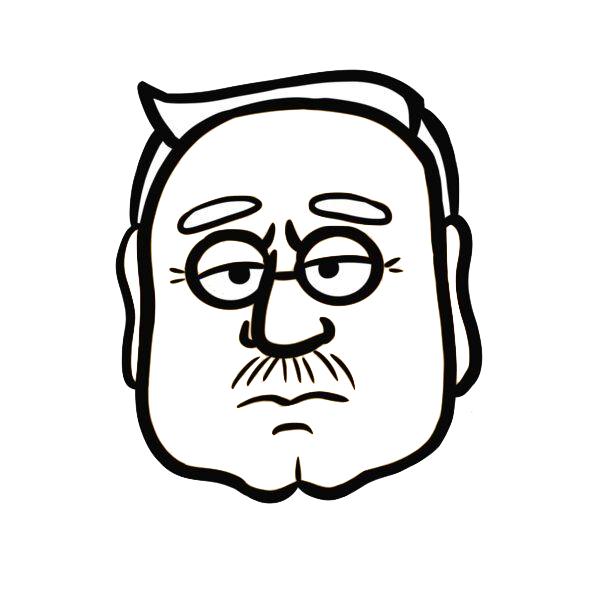
\includegraphics[width=7.5mm,height=7.5mm]{adler1.png} } & \getIndex{arr}{8}{4} & \getIndex{arr}{8}{5} \\ \hline
        \getIndex{arr}{9}{1} & \getIndex{arr}{9}{2} & \getIndex{arr}{9}{3}                         & \getIndex{arr}{9}{4} & \getIndex{arr}{9}{5} \\ \hline
        \getIndex{arr}{10}{1} & \getIndex{arr}{10}{2} & \getIndex{arr}{10}{3}                         & \getIndex{arr}{10}{4} & \getIndex{arr}{10}{5} \\ \hline
      \end{tabularx}%
    } \\
\end{tabularx}
\end{document}
